\documentclass[a4 paper,12pt]{article}

\usepackage[margin=2cm]{geometry}
\usepackage{setspace}
\usepackage[rgb]{xcolor}
\usepackage{verbatim}
\usepackage{subcaption}
\usepackage{amsgen,amsmath,amstext,amsbsy,amsopn,tikz,amssymb,tkz-linknodes}
\usepackage{fancyhdr}
\usepackage[colorlinks=true, urlcolor=blue,  linkcolor=blue, citecolor=blue]{hyperref}
\usepackage[colorinlistoftodos]{todonotes}
\usepackage{rotating}

\hypersetup{
    pdfauthor={Diego Cánez},
    pdftitle={Lab 5},
    pdfkeywords={Networks},
    pdfcreator={PDFLaTeX},
    pdfproducer={PDFLaTeX},
}

\usepackage[english]{babel}
\usepackage[utf8]{inputenc}
\usepackage{booktabs}

\newcommand{\ra}[1]{\renewcommand{\arraystretch}{#1}}

\newcommand{\homework}[6]{
    \pagestyle{plain}
    \newpage
    \setcounter{page}{1}
    \noindent
    \begin{center}
    \framebox{
        \vbox{\vspace{3mm}
        \hbox to 6.5in { {\bf CS2901~Networking and Communication \hfill {\small #2}} }
        \vspace{7mm}
        \hbox to 6.5in { {\Large \hfill #1  \hfill} }
        \vspace{7mm}
        \hbox to 6.5in { {{\rm #3} \hfill} {\rm #4} }
        \vspace{3mm}}
    }
   \end{center}
   \vspace*{6mm}
}

\newcommand{\problem}[2]{~\\\fbox{\textbf{Problem #1}}\hfill #2 \newline\newline}
\newcommand{\subproblem}[1]{~\newline\textbf{(#1)}}
\newcommand{\solution}{~\newline\textbf{\textit{(Solution)}} }

\renewcommand*{\thesection}{\Roman{section}}

\usepackage{graphicx}
\usepackage{placeins}
\usepackage{hyperref}
\usepackage{graphicx}
\usepackage[english]{babel}
\renewcommand{\figurename}{Fig.}
\addto\captionsenglish{%
  \renewcommand{\figurename}{Fig.}%
  \renewcommand{\contentsname}{Table of Contents}%
}
\usepackage{listings}
\usepackage{xcolor}
 
\definecolor{codegreen}{rgb}{0,0.6,0}
\definecolor{codegray}{rgb}{0.5,0.5,0.5}
\definecolor{codepurple}{rgb}{0.58,0,0.82}
 
\lstdefinestyle{mystyle}{
    commentstyle=\color{codegreen},
    keywordstyle=\color{magenta},
    numberstyle=\tiny\color{codegray},
    stringstyle=\color{codepurple},
    basicstyle=\ttfamily\footnotesize,
    breakatwhitespace=true,
    breaklines=true,                 
    captionpos=b,                    
    keepspaces=true,                 
    numbers=left,                    
    numbersep=5pt,                  
    showspaces=false,                
    showstringspaces=false,
    showtabs=false,                  
    tabsize=2
}
 
\lstset{style=mystyle}

\begin{document}
\homework{Lab 5: Grakn}{\today}{Diego Cánez}{University of Engineering and Technology}{}

\section{Introduction}

Grakn is a service for knowledge-oriented systems, that manages informations through as an entity-relationship model. It includes native algorithms for performing inference on the data and allows for more flexible storage of data.

Trying out Grakn, I was reminded of an area in Artificial Intelligence called Knowledge Representation and Reasoning (KR\&R) that caught my attention some months ago. It was interesting to try out some of those concepts through Grakn's intuitive command line utilities and integration with popular programming languages like Python.

Although the assignment required only to create a social network schema and play with it, I wanted to test Grakn's power in real-life data. With this in mind, I challenged myself to build what I called a "potential-friends-network". The concepts is very simple: If I follow someone and that person also follows me back, than I'm (probably) his friend. If that person is a friend (mutual-follow) with another person, then there are considerable chances I can get to know that person. 

The question was, uninevitable: Who could I be friends with? Could I possibly meet a prestiguous academic in the research areas I enjoy?

\section{Setup}

\subsection{Twitter's API}

Setting up a Twitter's Developer Account is fairly easy, but it gets a little bit more complicated once you have to create an "App". Apps provide the credentials you need for your application but require a Website with SSL certification for authentication. My go-to choice was a DigitalOcean Ubuntu 18 Droplet, a Namecheap domain and a Comodo SSL Certificate. 

\subsection{Grakn Schema}

For convinience, I kept the Grakn Schema as simple as I could. This was the result:

\FloatBarrier
\textbf{The Grakn Schema for Twitter Followers} \texttt{twitter/schema.gql}\par\medskip
    \lstinputlisting{../twitter/schema.gql}
\FloatBarrier

To set Grakn first run \texttt{grakn server start} and then \texttt{grakn console --keyspace twitter --file twitter/schema.gql} to load the schema.

\subsection{Python Scripting}

Twitter's API and some related utilities were handled through \texttt{twitter-controller.py}. An example of this was the \texttt{get\_next\_mutuals} function, which returned the mutual-follows of a given node by taking the intersection between the people that follow a certain person a the people that are followed by that person.


The \texttt{graph.py} file handled the graph algorithms such as generic implementations DFS and BFS. These were depth-limited because the Twitter Free API only allowed for 15 requests in 15 minutes, which was basically nothing.

The \texttt{main.py} file handled the connection with the Grakn Server and defined some functions to be ran as the DFS traversed the graph formed previously. \texttt{grakn-write} binded some local parameters and took a node instance and committed it to Grakn.



\section{Results}

\FloatBarrier
\begin{figure}
\centering
\textbf{Inserting Friendship relations}\par\medskip
    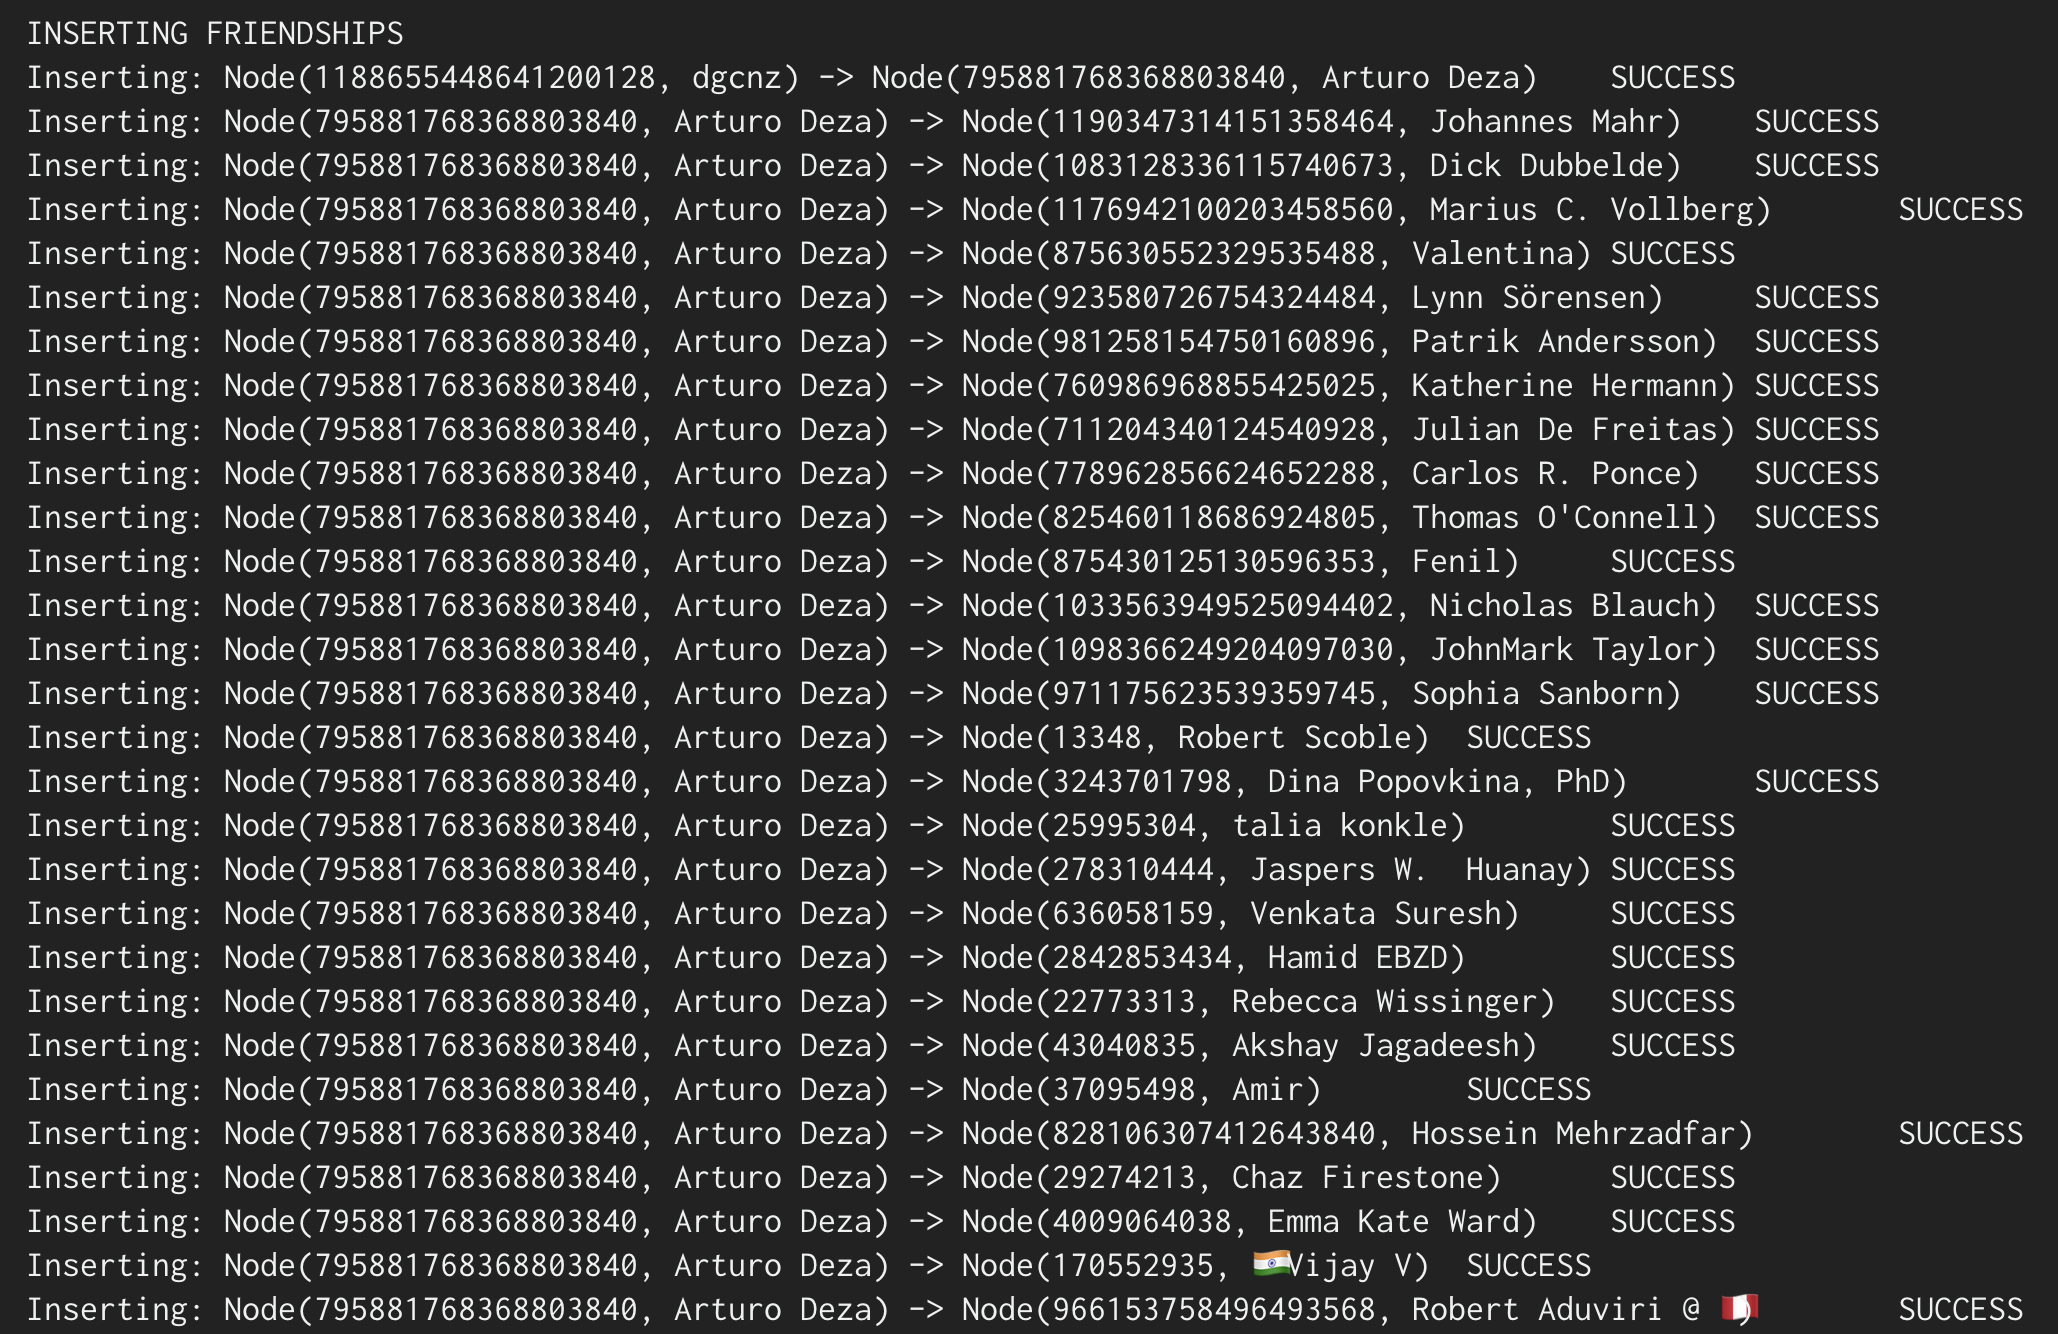
\includegraphics[scale=0.30]{figures/success.png}
\caption {A sample of the mutual-followers network.}
\end{figure}
\FloatBarrier

\FloatBarrier
\begin{figure}
\centering
\textbf{My potential acquaintances}\par\medskip
    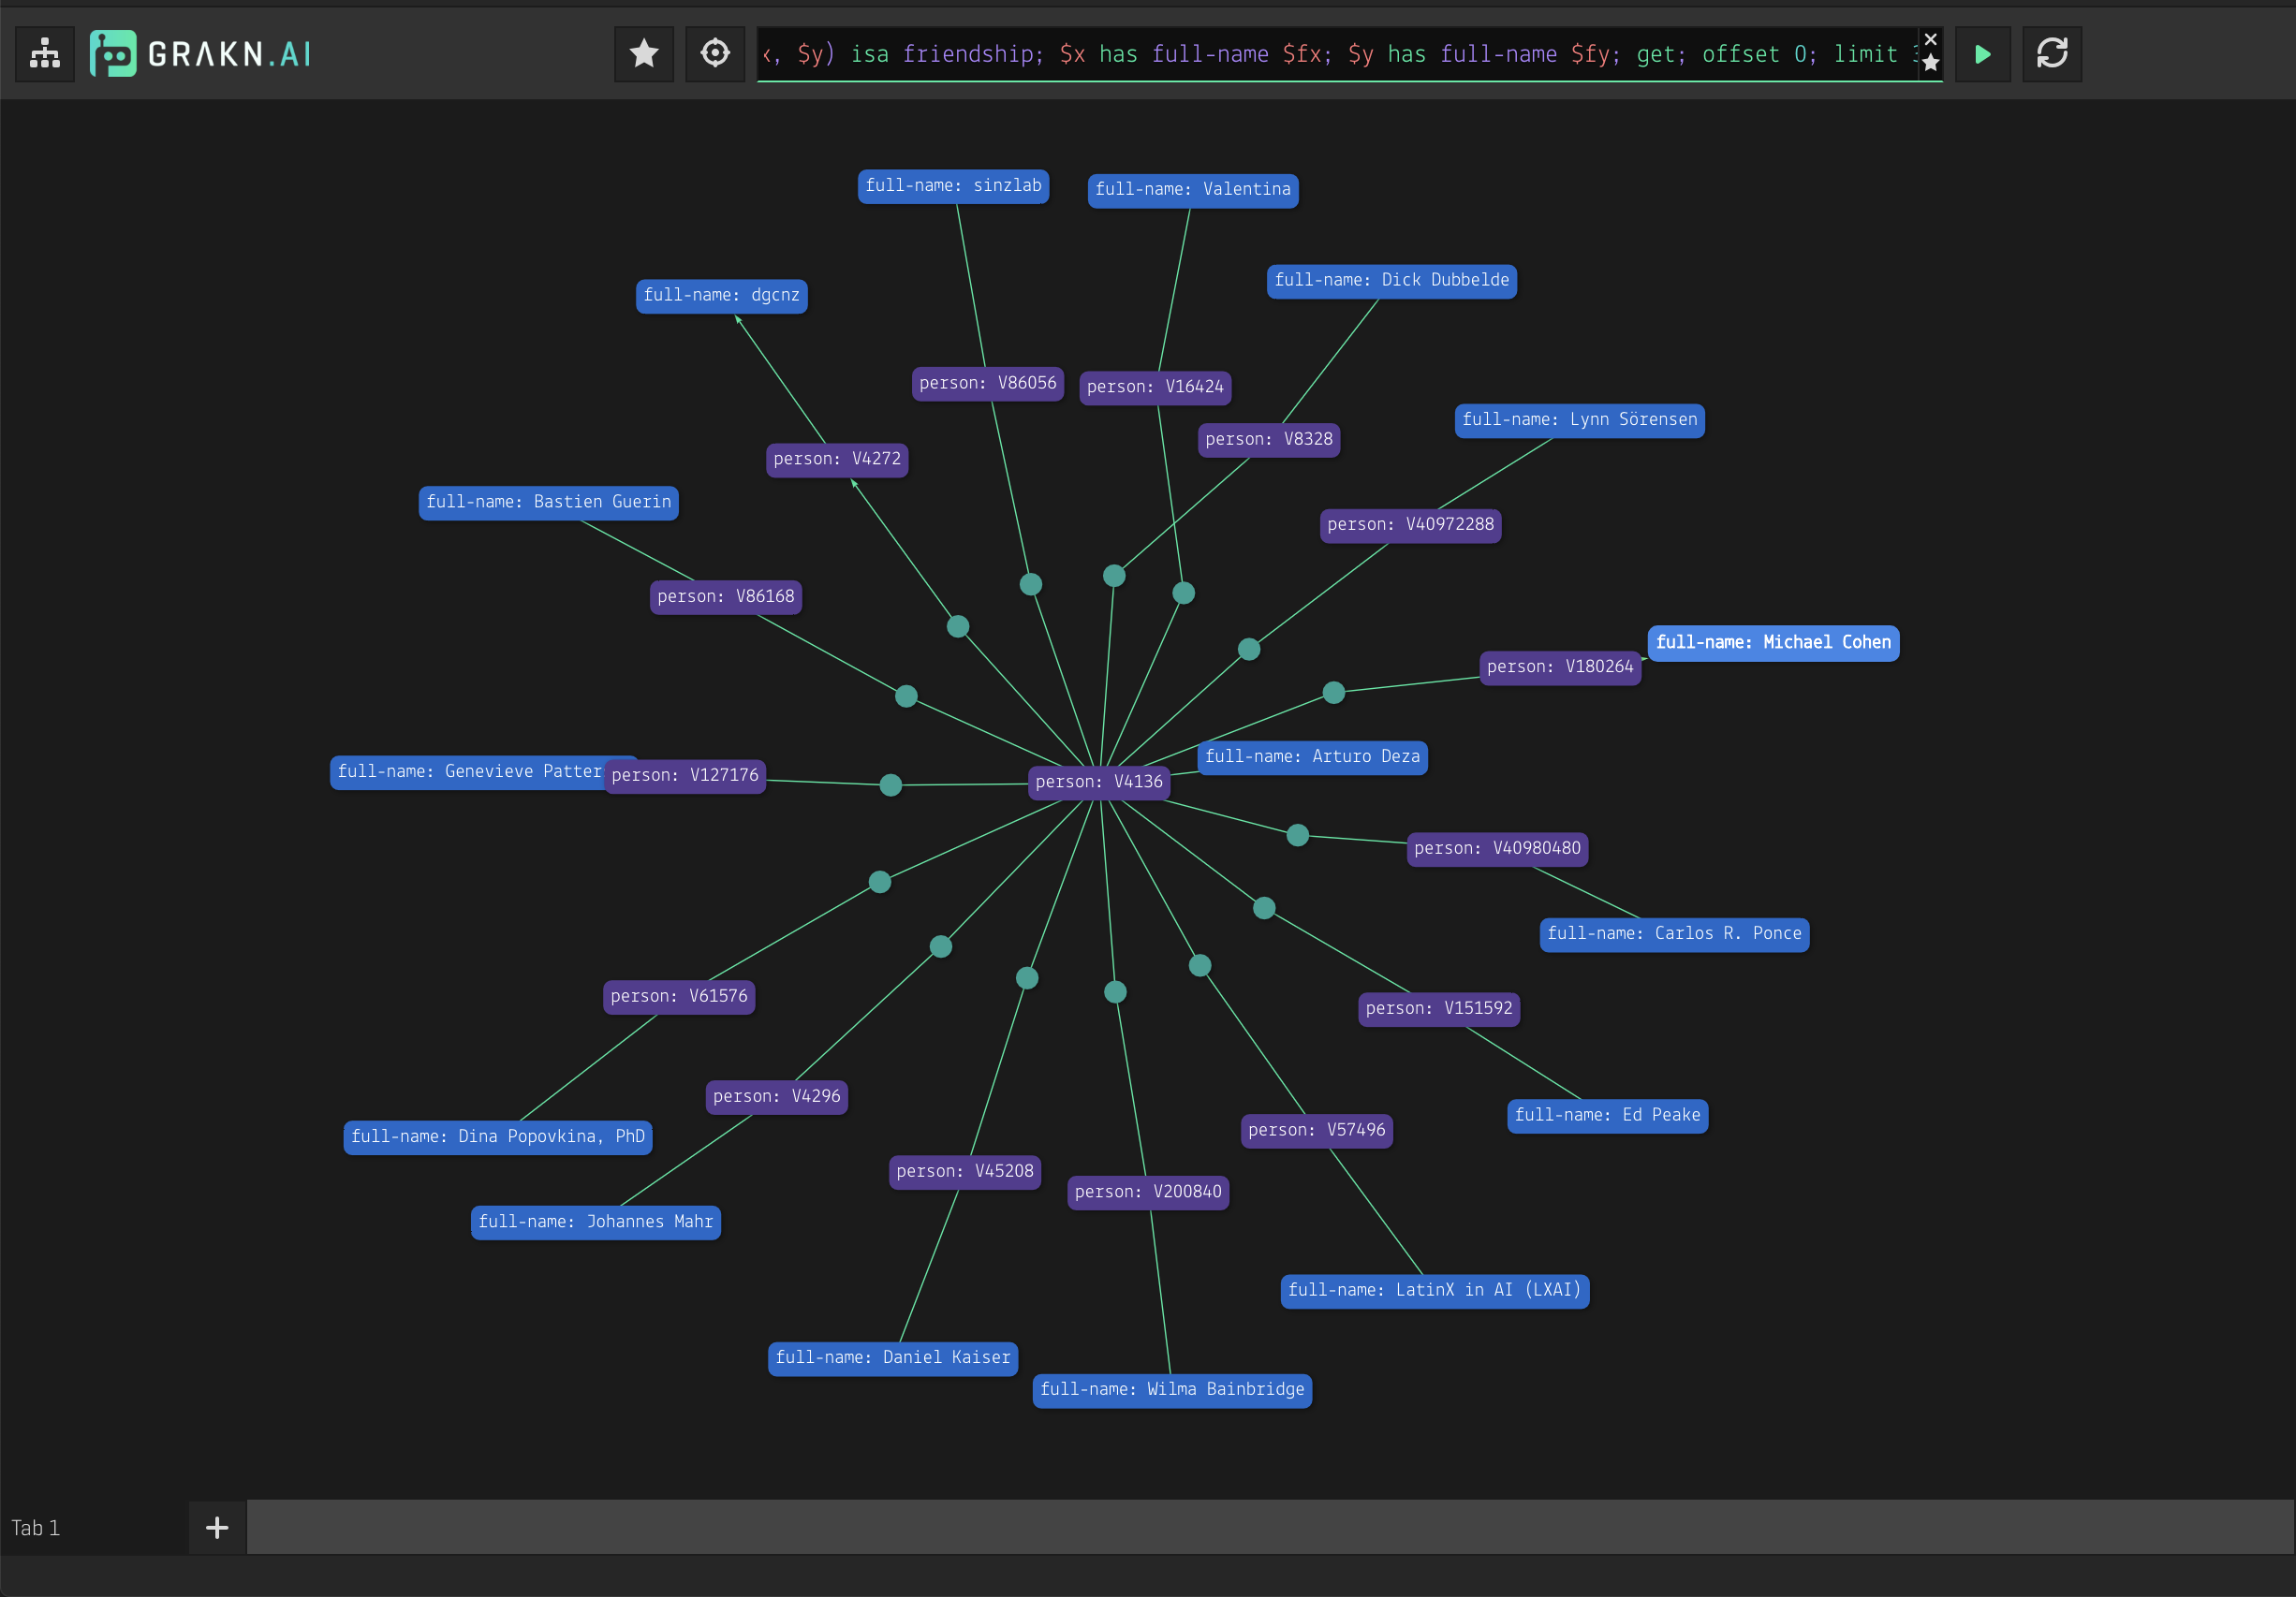
\includegraphics[scale=0.30]{figures/grakn-workbase.png}
\caption {A sample of the mutual-followers network.}
\end{figure}
\FloatBarrier

Overall, the result was interesting and the following figure of the Grakn Workbase shows such work.

My potential acquaintances graph was promising. A few months ago, I had met a PhD candidate in AI called Arturo Deza and such connection is clearly seen as the strongest one. Probably because of his success, he had a lot of mutual-follows (such quantity can't be clearly seen because of the \texttt{limit 30} query) and that meant that I \textit{could}, in theory, be friends with those people. It was a fun experiment, but the Twitter API Request Rate Limit didn't allow me to progress further than this.


\section{Appendix}

\FloatBarrier
\bigbreak
\noindent \textbf{Graph Utilities and Algorithms}\par\medskip
    \lstinputlisting{../graph.py}
\FloatBarrier

\FloatBarrier

\bigbreak
\noindent \textbf{Twitter API Controller}\par\medskip
    \lstinputlisting{../twitter_controller.py}
\FloatBarrier

\FloatBarrier
\bigbreak
\noindent \textbf{Main Program}\par\medskip
    \lstinputlisting{../main.py}
\FloatBarrier

\end{document}
